Проблема Борсука: $\Omega \subset \R^n, diam \Omega = sup_{x, y \in \Omega} |x - y| < \infty$.

Borsuk, 1933: $\Omega = \Omega_1 \sqcup \Omega_2 \sqcup \dots \sqcup \Omega_f$, $diam \Omega_i < diam \Omega$, $f(\Omega) = $ min число частей, на которое можно разбить $\Omega$; $f(n) = max_{\Omega} f(\Omega)$.

б.о.о. можно считать, что $diam \Omega = 1$, т.к. остальные мы тогда тоже научимся получать; $\Omega$ можно считать замкнутым, так как от точек на границе не поменяется диаметр. Более того, можно даже считать выпуклым (брать выпуклую оболочку), строгое док-во не нужно.

На прямой ($\R$): очевидно, берём $\Omega$, накрываем отрезком длины 1, разделяем пополам, очевидно, что диаметр стал меньше. Таким образом, $f(1) = 2$.

На плоскости ($\R^2$): очевидно, что $f(2) \geqslant 3$: берём 3 точки, которые вершины равностороннего треугольника (аналогично доказывается, что $f(n) \geqslant n + 1$).

Докажем, что $f(2) \leqslant 3$. 

\Statement Любое выпуклое множество диаметра 1 можно загнать в шестиугольник с расстоянием между противоположными сторонами 1. (термин: покрышка)

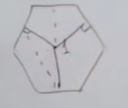
\includegraphics[]{images/72.JPG} 

И вот этими расстояниями она разбивается на три части, диаметры которых меньше 1.

\Proof

Возьмём произвольную прямую, не имеющую общих точек с $\Omega$. Строим параллельную ей прямую, которая бы касалась с $\Omega$ и ещё одну, как бы с 2х сторон. С этим всё хорошо, т.к. мн-во выпуклое. Далее достраиваем это до шестиугольника с углами по 120 градусов, а расстояние между параллельными сторонами не более 1.

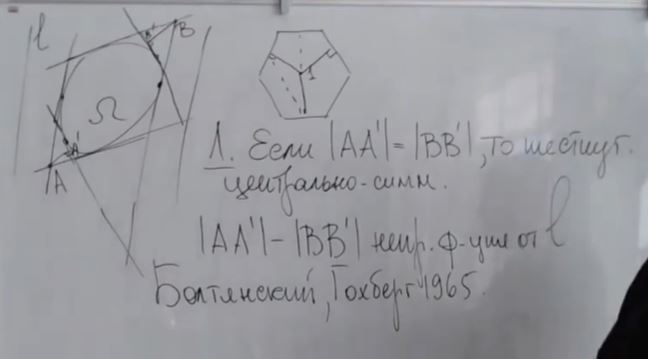
\includegraphics[]{images/72_3.JPG}

Таким образом, раз функция этих расстояний непрерывна и в начале больше 0, а в конце меньше 0, то будет такое положение прямой $l$, когда значение функции равно 0, значит, мы получим правильный шестиугольник.

\EndProof